It follows from the discussion above, that full Gaussian process regression scales as $O(n^3)$ and thus cannot be applied to big datasets. In this section we will review several approximate methods, that make Gaussian processes practical.

\subsection{Methods, based on inducing inputs}
	Most of the existing methods are based on introducing a set of $m$ function points that are called inducing inputs. Using these inputs one can make approximate predictions of the values of the hidden process at test points with a complexity of $O(nm^3)$ instead of $O(n^3)$.
	
	Consider the following situation. We have a dataset of $n$ examples $x_i$ with corresponding values $y_i$. We will denote the matrix of pairwise values of the covariance function by $K_{nn}$. Now we introduce a set of $m$ inducing inputs. We will denote the corresponding covariance matrix by $K_{mm}$ and the matrices of covariances between the inducing points and training points by $K_{nm}$ and $K_{mn}$. We will denote the vectors, comprised of noisy and true function values $y_i$ and $f_i$ at training points by $y$ and $f$ respectively. We will also introduce a distribution $q(u)$ over the hidden function values $u$ at the inducing inputs.
	
	It's easy to see, that
	$$p(y|f) = \N (y|f, \sigma_n I),$$
	$$p(f|u) = \N (f|K_{nm} K_{mm}^{-1}u, \tilde K),$$
	$$p(u) = \N(u|0, K_{mm}),$$
	where $\tilde K = K_{nn} - K_{nm} K_{mm}^{-1} K_{mn}.$
		
	\subsubsection{Variational learning of inducing points}
		\label{Titsias}
		
		The method discussed here was introduced in \cite{Titsias}. This method provides a way to find the optimal positions of the inducing points, as well as the optimal distribution of the process value at these points.

		Let $z$ denote a vector comprized of the process values at some new points. We can calculate the predictive distribution at these points as follows
		$$p(z|y) = \int p(z|f) p(f|y) df.$$
		Let's fix the inducing point positions $x_1, \ldots, x_m$. As above, $u$ is the vector compised of the process values at these points. We can rewrite the above equation
		\begin{equation}
			\label{predictive1}
			p(z|y) = \iint p(z|u, f) p(f| u, y) p(u|y)df du,
		\end{equation}
		% $$p(z | y) = \iint p(z | u, f) p(f | u, y)df du,$$
		as $p(z|u, f, y) = p(z|u, f)$. 

		Suppose for a moment, that $u$ is a sufficient statistics for the parameter $f$ in the scence that $z$ and $f$ are conditionally independent given $u$. Then we have 
		$$p(z|f, u) = \frac {p(z, f|u)} {p(f|u)} = \frac {p(z | u) p(f | u)}{p(f|u)} = p(z|u),$$
		$$p(z|y, u) = \frac {p(z, y, u)}{p(y, u)} = \frac {\int p(y|f)p(f, z, u) du}{\iint p(y|f) p(f, z, u) df dz} = \frac {\int p(y|f) p(z|u) p(u|f) p(f)df}{\iint p(y|f) p(z|u) p(u|f) p(f)df dz} = $$
		$$= \frac {\int p(y|f)p(f)p(u|f)df \cdot p(z|u)} {\int p(y|f)p(f)p(u|f)df \cdot \int p(z|u) dz} = \frac{\int p(y, f) p(u|f) df} {\int p(y, f) p(u|f) df} p(z|u) = p(z|u).$$

		So, $p(z|y, u) = p(z|u)$. If we set the points, corrwsponding to the process values $z$, to the traing points, we will have $z = f$, and thus $p(f|y, u) = p(f|u)$.

		Substituting these formulas into (\ref{predictive1}) we achieve
		$$q(z) = p(z|y) = \iint p(z|u) p(f|u) p(u|y)df du = \iint p(z|u) p(u|y) du = $$
		\begin{equation}
			\label{predictive2}
			= \int p(z|u)\varphi(u) du  = \int q(z, u) du, 
		\end{equation}
		where $\varphi(u) = p(u|y)$, $q(z, u) = p(z|u)\varphi(u)$.

		In practice however it's difficult to guarantee that $u$ is a sufficient statistics. Thus we can only expect $q(z)$ to be an approximation to $p(z|y)$. In such case we can choose $\varphi(u)$ to be a variational distribution, where in general $\varphi(u) \ne p(u | y)$. We will consider $\varphi(u)$ to be Gaussian with a mean vector $\mu$ and covariance matrix $\Sigma$.

		By using the eq. (\ref{predictive2}) we can calculate the approximate posterior GP mean at point $x$ and covariance at points $x, x'$
		$$\E[z(x)] = K_{xm} K_{mm}^{-1} \mu,$$ 
		$$\cov(z(x), z(x')) = k(x, x') - K_{xm} K_{mm}^{-1} K_{mx'} + K_{xm} A K_{mx'},$$
		where $A = K_{mm}^{-1} \Sigma K_{mm}^{-1}$.

		Now we have to specify a way to find the variational distribution parameters $\mu$ and $\Sigma$, and the inducing input positions $X_m$ and a way to optimize the kernel hyper-parameters. 
		% In order to do so, we will form the variational distribution $q(f)$ and the exact posterior $p(f|y)$ on the training function values, and then minimize the distance between this two distributions. Equivalently, we can minimize a distance, between the augmented true posterior $p(f, u|y)$ and $q(f, u)$.
		In order to do so, we will form the variational distribution $q(f, u)$ and the exact posterior $p(f, u|y)$ on the training function values and the values at the inducing points, and then minimize the KL-divergence between these two distributions. This minimization is equivalently expressed as the maximization of the following lower bound of the true marginal likelihood:
		$$F_V(X_m, \varphi) = \iint p(f|u) \varphi(u) \log \frac{p(y|f) p(u)}{\varphi(u)} df du.$$
		This bound can be optimized analytically with respect to $\phi$. The optimal distribution $\varphi(u) \sim \N(u|\hat u, \Lambda^{-1})$, where
		$$\Lambda = \frac 1 {\sigma_n} K_{mm}^{-1} K_{mn} K_{nm} K_{mm}^{-1} + K_{mm}^{-1},$$
		$$\hat u = \frac 1 {\sigma_n} \Lambda^{-1} K_{mm}^{-1} K_{mn} y.$$
		Substituting the optimal values of variational parameters into the $F_V$ we obtain the following bound
		$$F_V(X_m) = \log \N(y|0, \sigma_n^2 I + K_{nm} K_{mm}^{-1} K_{mn}) - \frac 1 {2\sigma_n^2} \tr(\tilde K).$$

		Another derivation of this lower bound is provided in section (\ref{svi}).

		The bound $F_V(X_m)$ is computed in $o(nm^2)$ time. Now we will calculate it's gradient in order to be able to maximize it with respect to $X_m$ and kernel hyper-parameters. We will denote $B = \sigma_n^2 I + K_{nm} K_{mm}^{-1} K_{mn}$. Then
		$$F_V(X_m, \theta, \sigma_n) = -\frac 1 2 \left(n \log 2\pi + \log |B| + y^T B^{-1} y + \frac 1 {\sigma_n^2} \tr(\tilde K)\right),$$
		$$\derivative{F_V}{\theta} = \frac 1 2 \left( -\tr \left(B^{-1} \derivative{B}{\theta}\right) + y^T B^{-1} \derivative{B}{\theta} B^{-1} y - \right.$$    
		$$- \left. \frac 1 {\sigma_n^2} \tr\left(\derivative{K_{nn}}{\theta} - \left(\derivative{K_{nm}}{\theta}K_{mm}^{-1} - K_{nm} K_{mm}^{-1} \derivative{K_{mm}}{\theta}K_{mm}^{-1}\right) K_{mn} - K_{nm} K_{mm}^{-1} \derivative{K_{mn}}{\theta}\right)\right),$$
		where
		$$\derivative{B}{\theta} = \left(\derivative{K_{nm}}{\theta}K_{mm}^{-1} - K_{nm} K_{mm}^{-1} \derivative{K_{mm}}{\theta}K_{mm}^{-1}\right) K_{mn} +  K_{nm} K_{mm}^{-1} \derivative{K_{mn}}{\theta}.$$

		We can rewrite
		$$\derivative{F_V}{\theta} = \frac 1 2 \left( -\tr \left(B^{-1} \derivative{B}{\theta}\right) + y^T B^{-1} \derivative{B}{\theta} B^{-1} y - \frac 1 {\sigma_n^2} \tr \left(\derivative {K_{nn}} {\theta} - \derivative {B}{\theta}\right) \right).$$

		Now we can optimize $F_V$ with respect to kernel hyper-parameters. Similarly, we can take derivatives with respect to $X_m$ and $\sigma_n$ and opptimize $F_V$ with respect to them as well.

		However, if we compute $F_v$ and it's derivatives as they are, it takes $O(n^3)$ time which is not faster, than recovering the full Gaussian process. So, we have to rewrite these values in a form that allows for faster computation.

		First of all, let's deal with $\log|B|$ and $B^{-1}$. Using the matrix determinant lemma we obtain
		$$|B| = |\sigma_n^2 I + K_{nm} K_{mm}^{-1} K_{mn}| = \frac{\left|K_{mm} + \cfrac{K_{mn} K_{nm}}{\sigma_n^2}\right| \sigma_n^2}{|K_{mm}|}.$$
		So, denoting $A = K_{mm} + \cfrac{K_{mn} K_{nm}}{\sigma_n^2}$, we obtain
		$$\log |B| = \log |A| + 2 \log \sigma_n - \log |K_{mm}|.$$
		Note tha this is computed in $O(n m^2)$ instead of $O(n^3)$.

		Using the Woodbury identity, we obtain
		$$B^{-1} = (\sigma_n^2 I + K_{nm} K_{mm}^{-1} K_{mn})^{-1} = \frac I {\sigma_n^2} - \frac{K_{nm} A^{-1} K_{mn}}{\sigma^{4}},$$
		which allows for computing $y^T B^{-1} y$ in $O(n m)$.

		Similarly, we can compute the gradient in $O(nm^2)$. In order to do so, we need to rewrite every trace $\tr(M_{nm} M_{mm} M_{mn})$, where $M_{kl} \in \R^{k \times l}$, in the form $\tr(M_{mm} M_{mn} M_{nm})$, which is computed in $O(nm^2)$, and use the derived formulas for $B^{-1}$.

		Now let's try to compute the second order derivatives.
		$$\frac{\partial^2 F_V} {\partial \theta_j \partial\theta_i} = \derivative{}{\theta_j} \left(\derivative{F_V}{\theta_i}\right) = \frac 1 2 \derivative{}{\theta_j} \left( -\tr \left(B^{-1} \derivative{B}{\theta_i}\right) + y^T B^{-1} \derivative{B}{\theta_i} B^{-1} y - \frac 1 {\sigma_n^2} \tr \left(\derivative {K_{nn}} {\theta_i} - \derivative {B}{\theta_i}\right)\right) = $$
		$$ = \frac 1 2 \left(\tr\left( B^{-1} \derivative{B}{\theta_j} B^{-1}\derivative{B}{\theta_i} - B^{-1} \sndderivative{B}{\theta_j}{\theta_i}\right) + y^T \left(B^{-1} \sndderivative{B}{\theta_j} {\theta_i} B^{-1}  - 2 B^{-1} \derivative{B}{\theta_j} B^{-1} \derivative{B}{\theta_i} B^{-1} \right) y \right. - $$
		$$ \left.- \frac 1 {\sigma_n^2} \tr\left(\sndderivative{K_{nn}}{\theta_j}{\theta_i} - \sndderivative{B}{\theta_j}{\theta_i}\right)\right),$$
		where
		$$\sndderivative{B}{\theta_j}{\theta_i} = \derivative{}{\theta_j} \left(\derivative{K_{nm}}{\theta_i}K_{mm}^{-1} K_{mn} - K_{nm} K_{mm}^{-1} \derivative{K_{mm}}{\theta_i}K_{mm}^{-1} K_{mn} +  K_{nm} K_{mm}^{-1} \derivative{K_{mn}}{\theta_i}\right) = $$

		$$ = \sndderivative{K_{nm}}{\theta_j}{\theta_i}K_{mm}^{-1} K_{mn} + K_{nm} K_{mm}^{-1}\sndderivative{K_{mn}}{\theta_j}{\theta_i}  - \derivative{K_{nm}}{\theta_i}K_{mm}^{-1} \derivative{K_{mm}}{\theta_j}K_{mm}^{-1}K_{mn} - $$
		
		$$- K_{nm} K_{mm}^{-1} \derivative{K_{mm}}{\theta_j}K_{mm}^{-1}\derivative{K_{mn}}{\theta_i} + \derivative{K_{nm}}{\theta_j}K_{mm}^{-1} \derivative{K_{mn}}{\theta_i} + \derivative{K_{nm}}{\theta_i} K_{mm}^{-1} \derivative{K_{mn}}{\theta_j} $$

		$$- \derivative{K_{nm}}{\theta_j} K_{mm}^{-1} \derivative{K_{mm}}{\theta_i}K_{mm}^{-1} K_{mn} + K_{nm} K_{mm}^{-1}\derivative{K_{mm}}{\theta_j} K_{mm}^{-1}\derivative{K_{mm}}{\theta_i}K_{mm}^{-1} K_{mn}$$

		$$ - K_{nm} K_{mm}^{-1} \sndderivative{K_{mm}}{\theta_j}{\theta_i}K_{mm}^{-1} K_{mn} + K_{nm} K_{mm}^{-1} \derivative{K_{mm}}{\theta_i}K_{mm}^{-1}\derivative{K_{mm}}{\theta_j}K_{mm}^{-1} K_{mn} - $$

		$$- K_{nm} K_{mm}^{-1} \derivative{K_{mm}}{\theta_i}K_{mm}^{-1} \derivative{K_{mn}}{\theta_j}.$$


	\pagebreak
	\subsubsection{Stochastic variational inference}
		In this subsection we describe a method for maximizing the lower bound (\ref{main_elbo}) in case of the GP-regression problem, which was proposed in \cite{BigData}. While the method, described in the previous section is much faster then the full GP-regression, it's complexity is still rather big. We could try, to reduce the time consumption of optimizing the lower bound, by using stochastic optimization methods. However, the function in the right hand side of (\ref{titsias_elbo}) does not have a form of sum over objects, and thus it's not clear, how to apply the stochastic methods.

However, the original bound from (\ref{main_elbo}) does have a form of sum over objects, and we can thus apply stochastic methods to it. In the regression case the bound looks like
$$\log p(y) \ge \sum_{i = 1}^{n} \left( \log \N(y_i | k_i^T K_{mm}^{-1} \mu, \sigma_n^2) - \frac 1 {2 \sigma_n^2} \tilde K_{ii} - \frac 1 2 \tr (\Sigma \Lambda_i) \right) - $$
$$ -\frac 1 2 \left (\log \frac {|K_{mm}|} {|\Sigma|} - m + \tr(K_{mm}^{-1} \Sigma) + \mu^T K_{mm}^{-1} \mu \right).$$

In the \lstinline{svi} method, we directly optimize this ELBO with respect to both variational parameters and kernel hyper-parameters in a stochastic way. The authors of the method suggest to use the stochastic gradient descent with natural gradients for the variational parameters and usual gradients for kernel hyper-parameters.

The natural gradients are the gradients with respect to the natural parameters of an exponential family of distributions. These gradients are considered to be effective in the case of optimization with respect to probability distribution parameters, because they use symmetrized $\mbox{KL}$ divergence between the distributions instead of usual distance between distribution parameters as a distance metric. For more information about natural gradients see for example \cite{ExpFamilyGeom}.

The complexity of computing a stochastic update of the variational and kernel parameters is independent of $n$ and scales as $\bigO(m^3)$. Thus, the stochastic optimization might give this method advantage against the \lstinline{vi} method. However, for big data problems the number of required inducing points $m$ is usually quite big. The number of parameters we have to optimize scales as $\bigO(m^2)$, which makes the optimization problem of the \lstinline{svi} method much harder then the one we have to solve in the \lstinline{vi} method. We will compare the two methods in the experiments section.


	\subsection{Stochastic variational inference for classification}
		The method described here was proposed in \cite{SVIclassification}. We could also apply the svi method to the classification problem. In order to do so, we will first rederive the ELBO from (\ref{L3}).

We will use the augmented model for the data.
$$p(y, f, u) = p(y | f) p(f | u) p(u).$$
\begin{figure}[!h]
	\centering
	\subfloat{
		\scalebox{0.7}{
			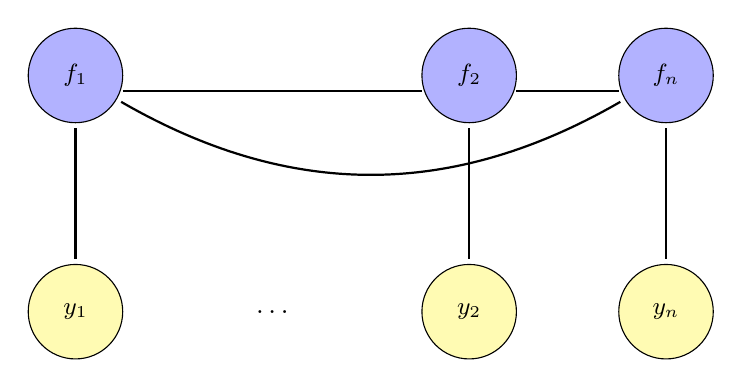
\begin{tikzpicture}
	\tikzstyle{x_i} = [circle, draw, fill=green!50, minimum size=1.2cm, text width=0.8cm, align=center, font=\large]
\tikzstyle{f_i} = [circle, draw, fill=blue!30, minimum size=1.2cm, inner sep=2pt, outer sep=2pt, font=\small, align=center]
\tikzstyle{y_i} = [circle, draw, fill=yellow!30, minimum size=1.2cm, inner sep=2pt, outer sep=2pt, font=\small, align=center]
\tikzstyle{edge_label} = [font=\small, label={[label distance = -4pt]90:$\text$}]
\tikzstyle{edge} = [thick, >=stealth]
\tikzstyle{biedge} = [thick, >=stealth]
\def\step{-3}
\def\layerpos{3}

% %data points
% \foreach \name/\x in {x_1/-2.5, x_2/2.5, x_n/5} 
%   	\node[x_i] (\name) at (\x, \layerpos) {$\name$};

% \node (other^1_1) at (0, \layerpos) {$\ldots$};

%latent process values
% \pgfmathsetmacro{\layerpos}{\layerpos + \step}

\foreach \name/\x in {f_1/-2.5, f_2/2.5, f_n/5} 
  	\node[f_i] (\name) at (\x, \layerpos) {$\name$};

% \node (other^2) at (0, \layerpos) {$\ldots$};
% \foreach \from/\to in {x_1/f_1, x_2/f_2, x_n/f_n}
% 	\draw[edge] (\from) -- (\to);

\draw[biedge] (f_1)++(0.6,-0.2) -- ++(3.8,0); %(f_2);
\draw[biedge] (f_2)++(0.6,-0.2) -- +(1.3,0);% ++ (f_n);
\draw [biedge] (f_1) to [out=-30,in=-150] (f_n);

%observables
\pgfmathsetmacro{\layerpos}{\layerpos + \step}

\foreach \name/\x in {y_1/-2.5, y_2/2.5, y_n/5} 
  	\node[y_i] (\name) at (\x, \layerpos) {$\name$};

\node (other^3) at (0, \layerpos) {$\ldots$};
\foreach \from/\to in {f_1/y_1, f_2/y_2, f_n/y_n}
	\draw[edge] (\from) -- (\to);
\end{tikzpicture}


		}
	}
	\hspace{1cm}
	\subfloat{
		\scalebox{0.7}{
			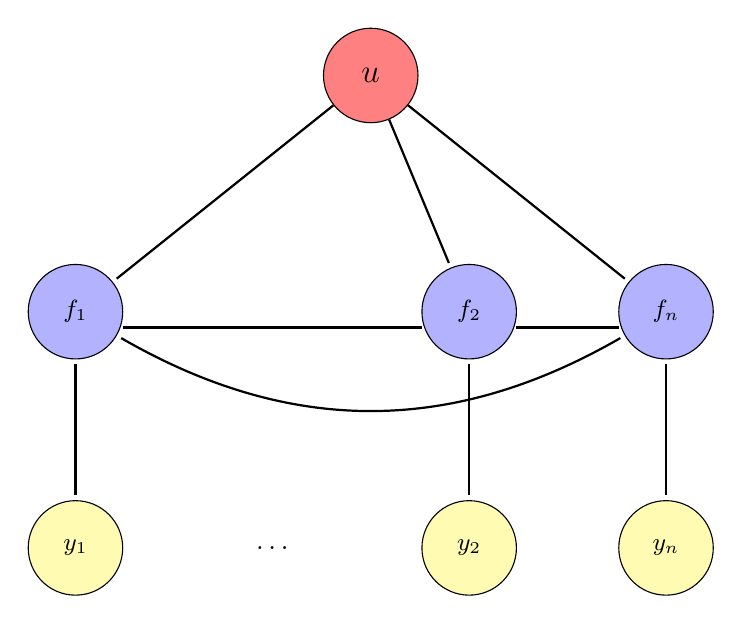
\begin{tikzpicture}
	\tikzstyle{u} = [circle, draw, fill=red!50, minimum size=1.2cm, text width=0.8cm, align=center, font=\large]
	\tikzstyle{x_i} = [circle, draw, fill=green!50, minimum size=1.2cm, text width=0.8cm, align=center, font=\large]
\tikzstyle{f_i} = [circle, draw, fill=blue!30, minimum size=1.2cm, inner sep=2pt, outer sep=2pt, font=\small, align=center]
\tikzstyle{y_i} = [circle, draw, fill=yellow!30, minimum size=1.2cm, inner sep=2pt, outer sep=2pt, font=\small, align=center]
\tikzstyle{edge_label} = [font=\small, label={[label distance = -4pt]90:$\text$}]
\tikzstyle{edge} = [thick, >=stealth]
\tikzstyle{biedge} = [thick, >=stealth]
\def\step{-3}
\def\layerpos{3}

% %data points
% \foreach \name/\x in {x_1/-2.5, x_2/2.5, x_n/5} 
%   	\node[x_i] (\name) at (\x, \layerpos) {$\name$};

% \node (other^1_1) at (0, \layerpos) {$\ldots$};

%latent process values
% \pgfmathsetmacro{\layerpos}{\layerpos + \step}

\foreach \name/\x in {f_1/-2.5, f_2/2.5, f_n/5} 
  	\node[f_i] (\name) at (\x, \layerpos) {$\name$};

% \node (other^2) at (0, \layerpos) {$\ldots$};
% \foreach \from/\to in {x_1/f_1, x_2/f_2, x_n/f_n}
% 	\draw[edge] (\from) -- (\to);

\draw[biedge] (f_1)++(0.6,-0.2) -- ++(3.8,0); %(f_2);
\draw[biedge] (f_2)++(0.6,-0.2) -- +(1.3,0);% ++ (f_n);
\draw [biedge] (f_1) to [out=-30,in=-150] (f_n);

%observables
\pgfmathsetmacro{\layerpos}{\layerpos + \step}

\foreach \name/\x in {y_1/-2.5, y_2/2.5, y_n/5} 
  	\node[y_i] (\name) at (\x, \layerpos) {$\name$};

\node (other^3) at (0, \layerpos) {$\ldots$};
\foreach \from/\to in {f_1/y_1, f_2/y_2, f_n/y_n}
	\draw[edge] (\from) -- (\to);
	\pgfmathsetmacro{\layerpos}{\step/2}
	\node[u] (inputs) at (1.25, 6) {$u$};

	\foreach \to in {f_1, f_2, f_n}
		\draw[edge] (inputs) -- (\to);
\end{tikzpicture}


		}
	}
	\caption{Graphical models for standard and inducing-point gaussian process classification}
\end{figure}

Applying the standard variational lower bound to this model, we obtain
$$\log p(y) \ge \E_{q(u, f)} \log \frac {p(y, u, f)}{q(u, f)} = \E_{q(u, f)}\log p(y | f) - \KL{q(u, f)} {p(u, f)}.$$
Our model implies $\E_{q(u, f)} \log p(y | f) = \E_{q(f)} \log p(y | f)$, where $q(f)$ is the marginal of $q(u, f)$.

We will consider the variational distributions of the following form:
$$q(u, f) = p(f | u) q(u),$$
where $q(u) \sim \N(u|\mu, \Sigma)$. This implies $q(f)$
$$q(f) = \int p(u | f) q(u) du = 
\N(f| K_{nm} K_{mm}^{-1} \mu, K_{nn} + K_{nm} K_{mm}^{-1}(\Sigma - K_{mm}) K_{mm}^{-1} K_{mn}).$$

Now, consider the KL-divergence in the lower bound we've devised.
$$\KL{q(u, f)} {p(u, f)} = \KL{q(u) p(f|u)} {p(u) p(f|u)} = \KL{q(u)} {p(u)}.$$

Finally, the lower bound is
\begin{equation}\label{sviELBO}
	\log p(y) \ge \E_{q(f)} \log p(y | f) - \KL{q(u)} {p(u)} = $$ $$ = \sum_{i = 1}^{n} \E_{q(f_i)} \log p(y_i | f_i) - \KL{q(u)} {p(u)},
\end{equation}
where 
$$q(f_i) = \N(f_i | k_i^T K_{mm}^{-1} \mu, K_{ii} + k_i^T K_{mm}^{-1} (\Sigma - K_{mm}) K_{mm}^{-1} k_{i}) = \N(f_i | m_i, S_i^2)$$
Note, that this lower bound is exactly the lower bound from (\ref{L3}), but now, we've derived it in a more general setting.

% Note, that 
% $$\E_{q(f_i)} \log p(y_i|f_i) = \E_{\N(f_i| m_i, S_i)} \log p(y_i|f_i) = \E_{\N(t | 0, 1)} \log p(y_i | (t \sqrt{S_i} + m_i))$$

Substituting the distributions $q$ and $p$ back into the (\ref{sviELBO}) we obtain

% $$\log p(y) \ge \sum_{i=1}^n \E_{\N(t | 0, 1)} \log p(y_i | t \sqrt{S_i} + m_i) -$$    
$$\log p(y) \ge \sum_{i=1}^n \E_{\N(f_i | m_i, S_i^2)} \log p(y_i | f_i) -$$
\begin{equation}\label{explicit_svi_elbo}
	-\frac 1 2 \left (\log \frac {|K_{mm}|} {|\Sigma|} - m + \tr(K_{mm}^{-1} \Sigma) + \mu^T K_{mm}^{-1} \mu \right) = L_3(\mu, \Sigma, \theta).
\end{equation}

Now we can maximize this lower bound with respect to variational parameters $\mu$, $\Sigma$ and covariance hyper-parameters $\theta$.

Let's find the derivatives of (\ref{explicit_svi_elbo}).

% $$\derivative{L_3}{\mu} = \sum_{i=1}^n \derivative{}{\mu} \E_{\N(t | 0, 1)} \log p(y_i | t \sqrt{S_i} + m_i) + K_{mm}^{-1} \mu = $$
$$\derivative{L_3}{\mu} = \sum_{i=1}^n \derivative{}{\mu} \left(\E_{\N(f_i | m_i, S_i^2)} \log p(y_i | f_i)\right) - K_{mm}^{-1} \mu = $$
$$ = \sum_{i=1}^n \derivative{}{m_i} \left(\E_{\N(f_i | m_i, S_i^2)} \log p(y_i | f_i)\right) \derivative{m_i}{\mu} - K_{mm}^{-1} \mu,$$
$$ = \sum_{i=1}^n \E_{\N(f_i | m_i, S_i^2)}\left[ \derivative{}{f_i} \log p(y_i | f_i)\right] \derivative{m_i}{\mu} - K_{mm}^{-1} \mu,$$

$$\derivative{L_3}{L_{\Sigma}} = \sum_{i=1}^n \derivative{}{S_i^2}\left( \E_{\N(f_i | m_i, S_i^2)} \log p(y_i | f_i)\right) \derivative{S_i^2}{L_{\Sigma}} + \hat L - K_{mm}^{-1} L_{\Sigma} = $$
$$= \frac 1 2 \sum_{i=1}^n \E_{\N(f_i | m_i, S_i^2)}\left[ \derivative{^2}{f_i^2} \log p(y_i | f_i)\right] \derivative {S_i^2}{L_{\Sigma}} + \hat L - K_{mm}^{-1} L_{\Sigma},$$
where
$$\hat L = 
\left(
\begin{array}{cccc}
\frac 1 {(L_{\Sigma})_{11}} & 0 & \ldots & 0\\
0 & \frac 1 {(L_{\Sigma})_{22}} & \ldots & 0\\
\ldots & \ldots & \ldots & \ldots\\
0 & 0 & \ldots & \frac 1 {(L_{\Sigma})_{mm}} \\
\end{array}   
\right) $$


$$\derivative{L_3}{\theta} = \derivative{}{\theta} \left(\sum_{i=1}^n \E_{\N(t | m_i, S_i^2)}  \log p(y_i | f_i)\right) -$$
$$- \frac 1 2 \tr\left(K_{mm}^{-1} \frac{\partial K_{mm}}{\partial \theta}\right) + \frac 1 2 \tr\left(\Sigma K_{mm}^{-1} \frac{\partial K_{mm}}{\partial \theta} K_{mm}^{-1} \right)+ \frac 1 2 \mu^T K_{mm}^{-1} \frac{\partial K_{mm}}{\partial \theta} K_{mm}^{-1}\mu.$$

Note that
$$\derivative{}{\theta} \left(\E_{\N(f_i | m_i, S_i^2)} \log p(y_i | f_i)\right) = \derivative{}{m_i}\left(\E_{\N(t | m_i, S_i^2)}  \log p(y_i | f_i) \right)\derivative{m_i}{\theta} + \derivative{}{S_i^2}\left(\E_{\N(f_i | m_i, S_i^2)}  \log p(y_i | f_i) \right)\derivative{S_i^2}{\theta} = $$
$$ = \E_{\N(f_i | m_i, S_i^2)} \left[\derivative{}{f_i} \log p(y_i | f_i) \right] \derivative{m_i}{\theta} + \frac 1 2 \E_{\N(f_i | m_i, S_i^2)} \left[\derivative{^2}{f_i^2} \log p(y_i | f_i) \right] \derivative{S_i^2}{\theta}$$

In order to compute the expectations in the derivatives, we can use the integral approximation techniques, and Gauss-Hermite quadrature in particular.

We will use logistic likelihood
$$\log p(y_i | f_i) =  - \log(1 + \exp( - y_i f_i)).$$

Then
$$\derivative{}{f_i} \log p(y_i | f_i) = \frac{y_i}{1 + \exp(y_i f_i)},$$
$$\derivative{^2}{f_i^2} \log p(y_i | f_i) = - \frac{y_i^2 \exp(y_i f_i)}{(1 + \exp(y_i f_i))^2}.$$

Now,
$$m_i = k_i^T K_{mm}^{-1} \mu,$$
$$\derivative{m_i}{\mu} = K_{mm}^{-1} k_i$$
$$\derivative{m_i}{\theta} = \derivative{k_i}{\theta}^T K_{mm}^{-1} \mu - k_i^T K_{mm}^{-1} \derivative{K_mm}{\theta} K_{mm}^{-1} \mu.$$
Finally, 
$$S_i^2 = K_{ii} + k_i^T K_{mm}^{-1} (L_\Sigma L_\Sigma^T - K_{mm}) K_{mm}^{-1} k_{i},$$
$$\derivative{S_i^2}{L_{\Sigma}} = 2 K_{mm}^{-1} k_i k_i^T K_{mm}^{-1} L_{\Sigma},$$
$$\derivative{S_i^2}{\theta} = \derivative{K_{ii}}{\theta} + 2 \derivative{k_i}{\theta}^T K_{mm}^{-1} (L_\Sigma L_\Sigma^T - K_{mm}) K_{mm}^{-1} k_{i}$$
$$ - 2 k_i^T K_{mm}^{-1} \derivative{K_{mm}}{\theta} K_{mm}^{-1} (L_\Sigma L_\Sigma^T - K_{mm}) K_{mm}^{-1} k_{i} - k_i^T K_{mm}^{-1} \derivative{K_{mm}}{\theta} K_{mm}^{-1} k_{i}.$$

The final formulas for the derevatives are
$$\derivative{L_3}{\mu} = \sum_{i=1}^n \E_{\N(f_i | m_i, S_i^2)}\left[\frac{y_i}{1 + \exp(y_i f_i)}\right] K_{mm}^{-1} k_i + K_{mm}^{-1} \mu,$$

$$\derivative{L_3}{L_{\Sigma}} = \sum_{i=1}^n \E_{\N(f_i | m_i, S_i^2)}\left[- \frac{y_i^2 \exp(y_i f_i)}{(1 + \exp(y_i f_i))^2} \right] K_{mm}^{-1} k_i k_i^T K_{mm}^{-1} L_{\Sigma} + \hat L - K_{mm}^{-1} L_{\Sigma},$$

$$\derivative{L_3}{\theta} = \sum_{i=1}^n \left[\E_{\N(f_i | m_i, S_i^2)} \left[\frac{y_i}{1 + \exp(y_i f_i)}\right] \left(\derivative{k_i}{\theta}^T K_{mm}^{-1} \mu - k_i^T K_{mm}^{-1} \derivative{K_mm}{\theta} K_{mm}^{-1} \mu \right)\right.$$
$$ + \frac 1 2 \E_{\N(f_i | m_i, S_i^2)} \left[- \frac{y_i^2 \exp(y_i f_i)}{(1 + \exp(y_i f_i))^2}\right] \left( \derivative{K_{ii}}{\theta} + 2 \derivative{k_i}{\theta}^T K_{mm}^{-1} (L_\Sigma L_\Sigma^T - K_{mm}) K_{mm}^{-1} k_{i} \right.$$
$$ \left.\left.- 2 k_i^T K_{mm}^{-1} \derivative{K_{mm}}{\theta} K_{mm}^{-1} (L_\Sigma L_\Sigma^T - K_{mm}) K_{mm}^{-1} k_{i} - k_i^T K_{mm}^{-1} \derivative{K_{mm}}{\theta} K_{mm}^{-1} k_{i} \right)\right]- $$
$$- \frac 1 2 \tr\left(K_{mm}^{-1} \frac{\partial K_{mm}}{\partial \theta}\right) + \frac 1 2 \tr\left(\Sigma K_{mm}^{-1} \frac{\partial K_{mm}}{\partial \theta} K_{mm}^{-1} \right)+ \frac 1 2 \mu^T K_{mm}^{-1} \frac{\partial K_{mm}}{\partial \theta} K_{mm}^{-1}\mu.$$






	\subsection{Variational inference for classification}
		We've described two approaches to optimizing the lower bound (\ref{explicit_svi_elbo}) in case of the regression problem. The optimization problem, that we have to solve in the \lstinline{svi} method seems to be much harder, than the one, that we have to solve in the \lstinline{vi} method, although we can solve the former with stochastic optimization techniques. In this subsection we will devise an approach, analogues to the \lstinline{vi-means} method for the classification problem.

The problem of optimizing the lower bound (\ref{explicit_svi_elbo}) with respect to the variational parameters $\mu$ and $\Sigma$ is very similar to the Bayesian logistic regression problem with Gaussian prior over the parameters. In \cite{JaakkolaJordan} a method, that implies a closed form approximation to the posterior distribution over the parameters. Applying this method, we can avoid optimization with respect to the variational parameters and use analytical formulas, similar to the ones, used in the \lstinline{vi-means} method.

Article \cite{JaakkolaJordan} provides the following lower bound for the logarithm of logistic function/.
$$\log g(x) = - \log(1 + \exp(-x)) \ge \frac x 2 - \frac \xi 2 + \log g(\xi) - \frac 1 {4 \xi} \tanh\left(\frac \xi 2 \right)(x^2 - \xi^2).$$
This bound becomes tight, when $\xi = x$.
We will denote $$\lambda(\xi) = \frac {\tanh\left(\frac\xi 2\right)}{4 \xi}.$$
This implies
$$\log g(x) \ge \frac x 2 - \frac \xi 2 + \log g(\xi) - \lambda(\xi) (x^2 - \xi^2)$$

Substituting this bound back to (\ref{explicit_svi_elbo}) we obtain
$$\log p(y) \ge \sum_{i = 1}^{n} \E_{q(f_i)} \log p(y_i | f_i) - \KL{q(u)} {p(u)} = \sum_{i = 1}^{n} \E_{q(f_i)} \log g(y_i f_i) - \KL{q(u)} {p(u)} \ge $$
$$\ge \sum_{i = 1}^{n}\left(\E_{q(f_i)} \left [\log g(\xi_i) + \frac {y_i f_i - \xi_i} {2} - \lambda(\xi_i) (f_i^2 - \xi_i^2) \right]\right) - \KL{q(u)} {p(u)} = $$
$$= \sum_{i = 1}^{n} \left(\log g(\xi_i) + \frac {y_i m_i - \xi_i} {2}  + \lambda(\xi_i) \xi_i^2 - \lambda(\xi_i) (m_i^2 + S_i^2) \right) - \KL{q(u)} {p(u)} = $$
$$= \sum_{i = 1}^{n} \left(g(\xi_i) - \frac {\xi_i}{2} + \lambda(\xi_i) \xi_i^2\right) + \frac 1 2 \mu^T K_{mm}^{-1} K_{mn} y - \tr\left(\Lambda(\xi) (K_{nn} + K_{nm} K_{mm}^{-1} (\Sigma - K_{mm}) K_{mm}^{-1} K_{mn})\right) -$$
$$- \mu^T K_{mm}^{-1} K_{mn} \Lambda(\xi) K_{nm} K_{mm}^{-1} \mu - \KL{q(u)} {p(u)} = J(\mu, \Sigma, \xi, \theta),$$
where 
$$\Lambda(\xi) = 
\left(
\begin{array}{cccc}
	\lambda(\xi_1) & 0 & \ldots & 0 \\
	0 & \lambda(\xi_2) & \ldots & 0 \\
	\ldots & \ldots & \ldots & \ldots \\
	0 & 0 & \ldots & \lambda(\xi_n) \\
\end{array}
\right).
$$

Differentiating $J$ with respect to $\mu$ and $\Sigma$ and setting the derivatives to zero, we obtain
\begin{equation}\label{vi_optimal_sigma}
	\hat \Sigma(\xi) = (2 K_{mm}^{-1} K_{mn} \Lambda(\xi) K_{nm} K_{mm}^{-1} + K_{mm}^{-1})^{-1},
\end{equation}
\begin{equation}\label{vi_optimal_mu}
	\hat \mu(\xi) = \frac 1 2 \hat \Sigma(\xi) K_{mm}^{-1} K_{mn} y.
\end{equation}
Note, that these formulas are very similar to the corresponding optimal values in the regression problem.

We now apply coordinate-wise optimization to tune both $\mu$, $\Sigma$ and $\xi$. On the first step we use formulas (\ref{vi_optimal_sigma}) and (\ref{vi_optimal_mu}) to find the optimal distribution over $f$ for the current values $\xi_{old}$ of $\xi$. On the second step we maximize $J$ with respect to $\xi$ for fixed $\mu$ and $\Sigma$. This leads to
$$\xi_i^2 = \E_{q(f | \xi_{old})} f_i^2 = m_i^2 + S_i^2.$$
Now, performing a few updates of $\mu$, $\Sigma$ and $\xi$, we obtain closed-form formulas for optimal
$\mu$ and $\Sigma$ and can substitute them back to the ELBO.

Note, that
$$\hat\Sigma(\xi) = K_{mm} B^{-1} K_{mm},$$
$$\hat\mu(\xi) = \frac 1 2 K_{mm} B^{-1} K_{mn} y,$$
where $B = 2 K_{mn} \Lambda(\xi) K_{nm} + K_{mm}$.

Maximizing our lower bound with respect to $\theta$ is equivalent to maximizing the following expression.
$$ \hat J(\theta) =  \frac 1 2 \mu^T K_{mm}^{-1} K_{mn} y - \tr\left(\Lambda(\xi) (K_{nn} + K_{nm} K_{mm}^{-1} (\Sigma - K_{mm}) K_{mm}^{-1} K_{mn})\right) -$$
$$ - \mu^T K_{mm}^{-1} K_{mn} \Lambda(\xi) K_{nm} K_{mm}^{-1} \mu -\frac 1 2 \left (\log \frac {|K_{mm}|} {|\Sigma|} + \tr(K_{mm}^{-1} \Sigma) + \mu^T K_{mm}^{-1} \mu \right) = $$
$$ = \frac 1 2 \mu^T K_{mm}^{-1} K_{mn} y - \mu^T K_{mm}^{-1}\left(K_{mn} \Lambda(\xi) K_{nm} + \frac 1 2 K_{mm} \right)K_{mm}^{-1}\mu + \frac 1 2 \log \frac {|\Sigma|}{|K_{mm}|} - $$
$$ - \tr\left(\Lambda(\xi) (K_{nn} - K_{nm} K_{mm}^{-1} K_{mn})\right) - \tr\left(K_{mm}^{-1} \Sigma K_{mm}^{-1} (K_{mn} \Lambda(\xi) K_{nm} + \frac 1 2 K_{mm})\right) = $$
$$ = \frac 1 4 y^T K_{nm} B^{-1} K_{mn} y - \frac 1 8 y K_{nm} B^{-1} K_{mn} y + \frac 1 2 \log |K_{mm}| - \frac 1 2 \log |B| - $$
$$ - \tr(\Lambda(\xi) \tilde K) - \frac 1 2 \tr(B^{-1} B) \propto $$
$$\propto \frac 1 8 y^T K_{nm} B^{-1} K_{mn} y + \frac 1 2 \log |K_{mm}| - \frac 1 2 \log |B| - \tr(\Lambda(\xi) \tilde K),$$
where $\tilde K = K_{nn} - K_{nm} K_{mm}^{-1} K_{mn}$.

Now, let's compute the derivatives of $\hat J$ with respect to $\theta$.

$$\derivative{\hat J}{\theta} = \frac 1 4 y^T \derivative{K_{nm}}{\theta} B^{-1} K_{mn} y - \frac 1 8 y^T K_{nm} B^{-1} \derivative{B}{\theta} B^{-1} K_{mn} y + $$
$$ + \frac 1 2 \tr\left(K_{mm}^{-1} \derivative{K_{mm}}{\theta}\right) - \frac 1 2 \tr\left(B^{-1} \derivative{B} {\theta}\right) - \tr \left(\Lambda(\xi) \derivative{\tilde K}{\theta}\right),$$
where
$$\derivative{\tilde K}{\theta} = \derivative{K_{nn}}{\theta} - 2 \derivative{K_{nm}}{\theta} K_{mm}^{-1} K_{mn} + K_{nm} K_{mm}^{-1} \derivative{K_{mm}}{\theta} K_{mm}^{-1} K_{mn},$$
$$\derivative{B}{\theta} = 4 \derivative{K_{mn}}{\theta} \Lambda(\xi) K_{nm} + \derivative{K_{mm}}{\theta}.$$

We can now iteratively optimize $J$ with respect to both variational parameters $\mu, \Sigma$ and kernel-hyperparameters $\theta$. On each iteration we perform several steps of tuning the variational parameters $\mu$, $\Sigma$ and $\xi$. Then, we optimize the obtained model $\hat J(\theta) \propto J(\mu, \Sigma, \xi, \theta)$ for fixed $\mu$, $\Sigma$ and $\xi$ with respect to $\theta$.

Recalculating $\mu$ and $\Sigma$ for fixed $\xi$ requires $\bigO(nm^2)$ operations. Updating $\xi$ for fixed $\mu$ and $\Sigma$ scales as $\bigO(nm^2)$ as well. Finally, calculating the ELBO $\hat J(\theta)$ and it's gradient requires $\bigO(nm^2)$.

The derived method is similar to both the Largange GP-classification and the \lstinline{vi} method.
